\documentclass[spanish]{scrartcl}
\usepackage[utf8]{inputenc}
\usepackage{babel}
\usepackage[headheight=47pt, paper=a4paper, top=3cm, left=2cm, right=2cm,bottom=3cm]{geometry}
\usepackage{tikz}
\usepackage{CIACcustom}
\usepackage{fourier}
\usepackage{amsmath, amsthm}
\usepackage{listings}
\usepackage{multicol}
\usepackage{fancyhdr}
\usepackage[urlcolor=blue, colorlinks]{hyperref}
\usepackage{booktabs,tabularx}
\usepackage{float}
\usepackage{wrapfig}
\usepackage[normalem]{ulem} %Para tachar palabras y hacer chistes ...

\newcolumntype{L}[1]{>{\hsize=#1\hsize\raggedright\arraybackslash}X}%
\newcolumntype{R}[1]{>{\hsize=#1\hsize\raggedleft\arraybackslash}X}%
\newcolumntype{C}[2]{>{\hsize=#1\hsize\columncolor{#2}\centering\arraybackslash}X}%

%% Cambiar las enumeraciones de numeros a enumeraciones de letras.
\renewcommand{\theenumi}{\Alph{enumi})}


\newcommand{\numCert}{1}
\newcommand{\annoCert}{2019}
\newcommand{\fechaCert}{6 de Abril de \annoCert}

\pagestyle{fancy}
\fancyhf{}
\rhead{\pgfimage[width=2.5cm]{imagenes/logo-ciac.png}}
\chead{
  Simulación Certamen \numCert\\
  IWI-131 Semestre I-\annoCert \\
  CIAC Casa Central
}
\lhead{\pgfimage[width=2.5cm]{imagenes/logo-usm.jpg}}
\rfoot{\LaTeXe / CIAC \annoCert}
\lfoot{\thepage}

\renewcommand{\ttdefault}{pcr}

\renewcommand{\footrulewidth}{0.4pt}% default is 0pt

%%% listings settings:
\definecolor{bggray}{rgb}{0.95,0.95,0.95}
\lstdefinestyle{consola}{
  backgroundcolor=\color{bggray},
  basicstyle=\small\ttfamily,
  frame=single,
  moredelim=[is][\bfseries]{[*}{*]},
  xrightmargin=5pt
}

\lstdefinestyle{mypy}{
  language=python,
  backgroundcolor=\color{bggray},
  basicstyle=\ttfamily\small\color{orange!70!black},
  frame=L,
  keywordstyle=\bfseries\color{green!40!black},
  commentstyle=\itshape\color{purple!40!black},
  identifierstyle=\color{blue},
  stringstyle=\color{red},
  numbers=left,
  showstringspaces=false,
  xrightmargin=5pt,
  xleftmargin=10pt
}

\newtheorem{CIACdef}{Definición}


\begin{document}
\section*{Programación - Certamen \numCert - \fechaCert}
\vspace*{-.6cm}
\begin{figure}[h]
    \centering
    
\includegraphics[scale=0.9]{Imagenes/nombrerol.png}
\end{figure}
\vspace*{-1.0cm}
\vspace*{-0.4cm}
\section*{Pregunta 1}

\begin{enumerate}
    \item A continuación se presenta el ruteo correspondiente:
\begin{center}
    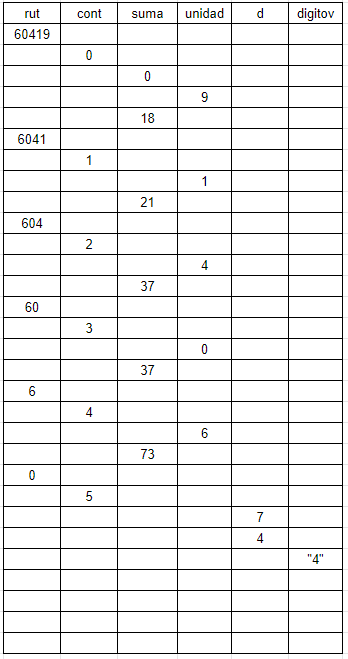
\includegraphics[scale=0.84]{Imagenes/ruteo_pauta}
\end{center}

    El programa imprime \texttt{4}.

    \item El código calculaba el dígito verificador del RUT. También era aceptable responder que, en base a cierto numero, este programa entrega un caracter que podría ser un dígito o una k.

\end{enumerate}

\newpage
\section*{Pregunta 2}

A continuación se presenta una forma posible de resolver el problema propuesto:
\lstinputlisting[
    style  = mypy,
    caption= \texttt{biblioteca.py}]{Code/p2.py}

\newpage
\section*{Pregunta 3}

A continuación se presenta una forma posible de resolver el problema propuesto:
\lstinputlisting[
    style  = mypy,
    caption= \texttt{tepyton.py}]{Code/p3.py}
\pagebreak[4]

\section*{Programación - Certamen \numCert - \fechaCert}
\vspace*{-.6cm}
\begin{figure}[h]
    \centering
    
\includegraphics[scale=0.9]{Imagenes/nombrerol.png}
\end{figure}
\vspace*{-1.0cm}
\section{Matrices}

Las funciones solicitadas y el máximo correspondiente (70600674) se calculan con el siguiente código

\lstinputlisting[style=mypy,caption=\texttt{matrices.py}]{Code/matrices.py}

\pagebreak[4]

\section*{Programación - Certamen \numCert - \fechaCert}
\vspace*{-.6cm}
\begin{figure}[h]
    \centering
    
\includegraphics[scale=0.9]{Imagenes/nombrerol.png}
\end{figure}
\vspace*{-1.0cm}
\section{Diccionarios}
\subsection{Algoritmo para contar cosas}
\lstinputlisting[style=mypy,caption=\texttt{contador.py}]{Code/contador.py}

\subsection{Signos zodiacales}
\lstinputlisting[style=mypy, caption=\texttt{contador.py}]{Code/signos.py}


\end{document}